
\heading{3. EXPERIMENTAL RESULTS}

Given the increased order of approximation, it is naturally expected
that some accuracy benefit could be gained by using a quintic spline
over a cubic spline. Experiments 1 and 2 below test some accuracy
differences between monotone cubic and quintic splines. Experiment 3
analyzes the number of operations performed by Algorithm
\ref{alg:monotone-spline} with increasingly large samples of monotone
data.

\heading{3.1 \enspace Approximating a Trigonometric Function}

For this experiment, the function $\sin(x) + x$ is considered over the
interval $[0,(5/2)\pi]$ as seen in Figure
\ref{fig:cubic_quintic_sin}. Given an increasing number of points, the
maximum error of cubic and quintic approximations is shown in Figure
\ref{fig:experiment_1}. The quintic approximation consistently has a
maximum error that is roughly half that of the cubic approximation,
given the same number of points. There is an increase in the error gap
between the two approximations as more points are added. The quintic
spline requires only $700$ points to approximate the function to the
same accuracy achieved by the cubic with $1000$ points.

%% \begin{figure}[h]
%%   \centering
%%   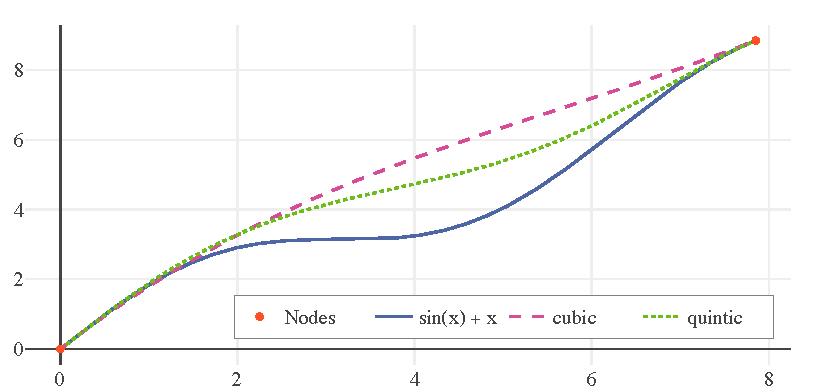
\includegraphics[width=.7\textwidth]{cubic-quintic-sin}
%%   \caption{Depicted above are the monotone cubic and quintic spline
%%   interpolants of the function $\sin(x) + x$ over the points $[0,
%%   (5/2) \pi]$.  Notice that the maximum error of the cubic
%%   interpolant is larger, because it only captures first derivative
%%   information at the points. The quintic interpolant captures both
%%   first and second derivative information at the points.}
%% \end{figure}

%% \begin{figure}
%%   \centering
%%   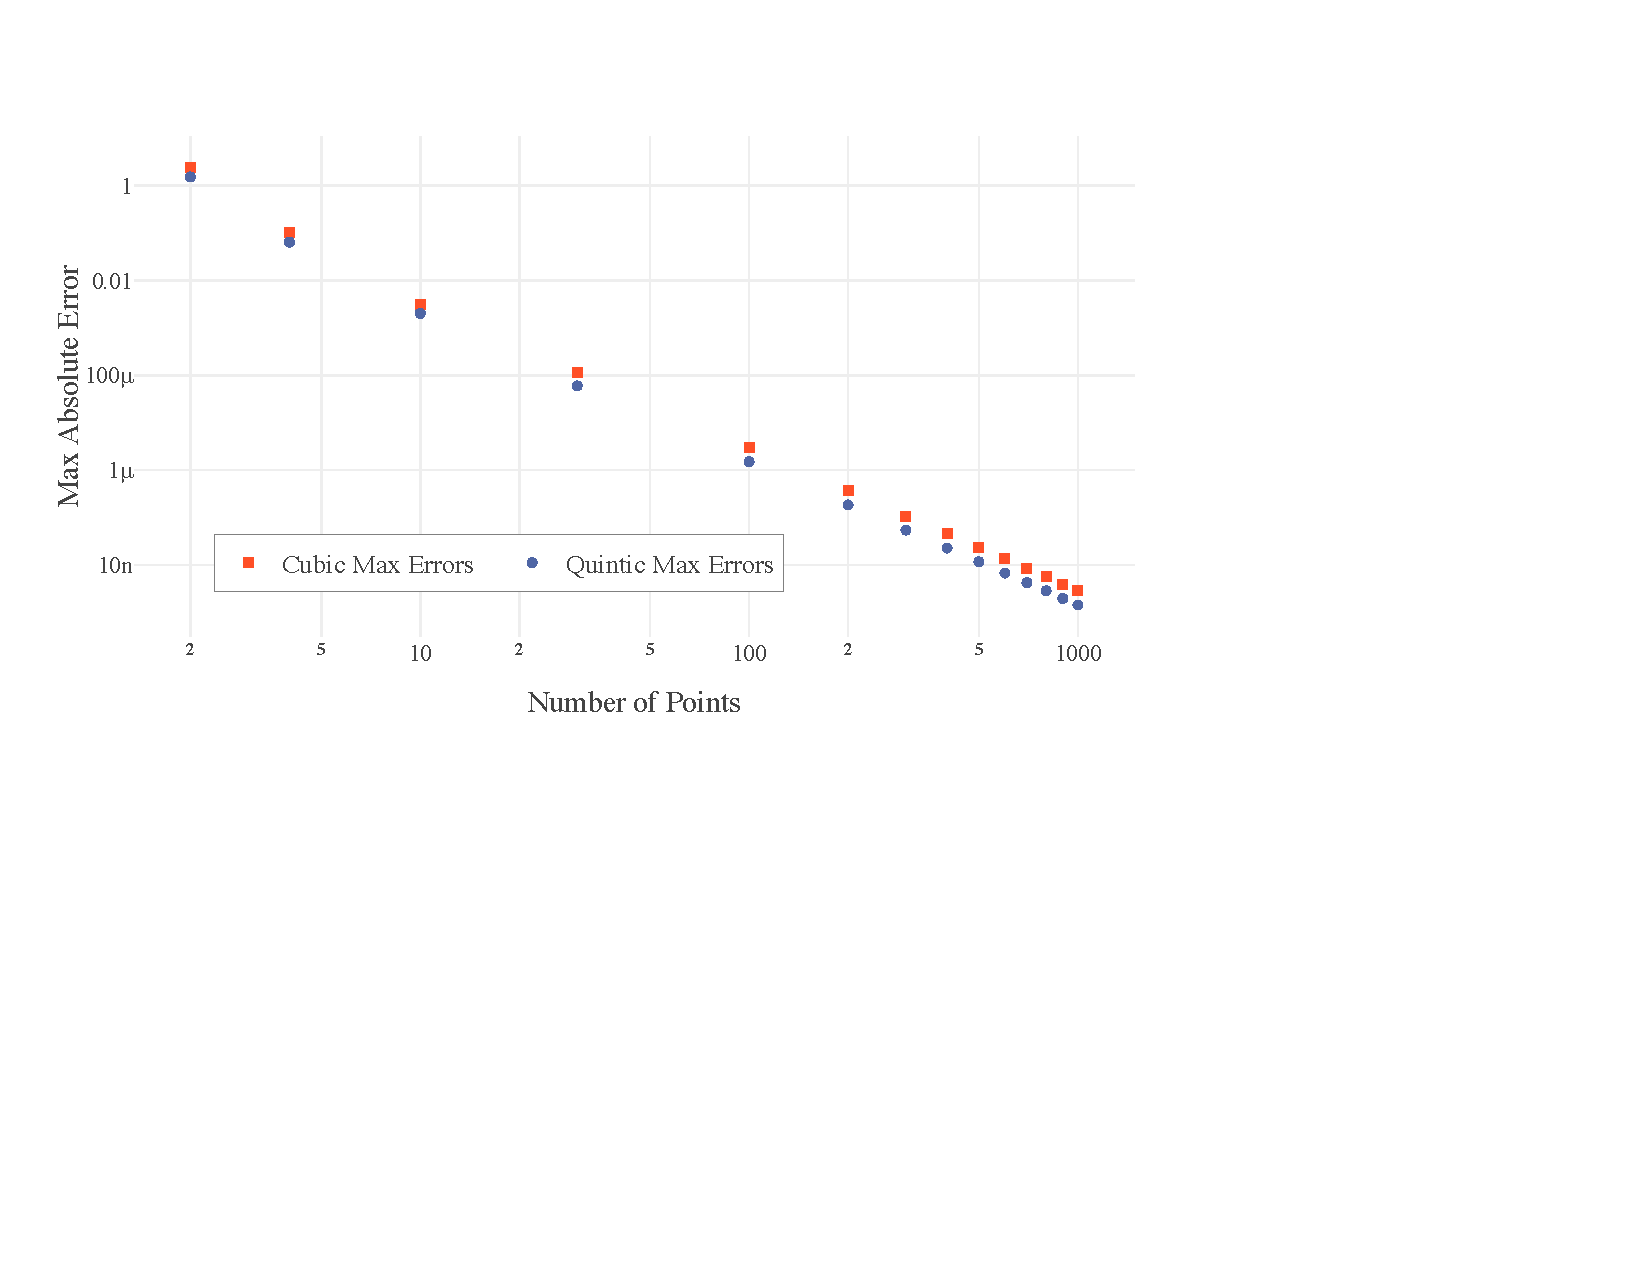
\includegraphics[width=.7\textwidth]{experiment_1_errors}
%%   \caption{The error in the quintic and cubic approximations of
%%   $\sin(x) + x$ with increasing number of points. Both axes are log
%%   scaled, where $\mu$ means $\times 10^{-6}$ and n means $\times
%%   10^{-9}$ on the vertical axis. The quintic approximation
%%   generally provides an approximation with about half of the
%%   maximum error of the cubic approximation, while the relative gap
%%   between grows with increasing number of points. In order to
%%   achieve the same absolute error the quintic spline requires ten
%%   fewer points at max error $10^{-4}$, thirty fewer points at max
%%   error $10^{-6}$, and $300$ fewer points at max error $10^{-8}$.}
%% \end{figure}

\heading{3.2 \enspace Random Number Generation}

Consider the cumulative distribution function (CDF) defined by a
mixture of three Gaussian distributions and visualized in Figure
\ref{fig:experiment_2_distribution}. The distributions have weights
$(.3, .6, .1)$, means $(.2, .45, .85)$ and standard deviations $(.05,
.08, .03)$. $200$ random samples are generated from this distribution
with both cubic and quintic approximations from four points, and over
$100$ trials the resulting spread of empirical distribution functions
(EDFs) are visualized in Figure \ref{fig:experiment_2_results}.

While an increased number of points could be used to decrease the
error in either approximation, the purpose of this experiment is to
demonstrate the effect approximation error has on random number
generation. The errors in the CDFs are magnified by the variance
involved in randomly sampling from a distribution. As a result, while
the cubic and quintic spline approximations have similar maximum
error, the cubic distribution is significantly distorted around the
first and second modes.

%% \begin{figure}
%%   \centering
%%   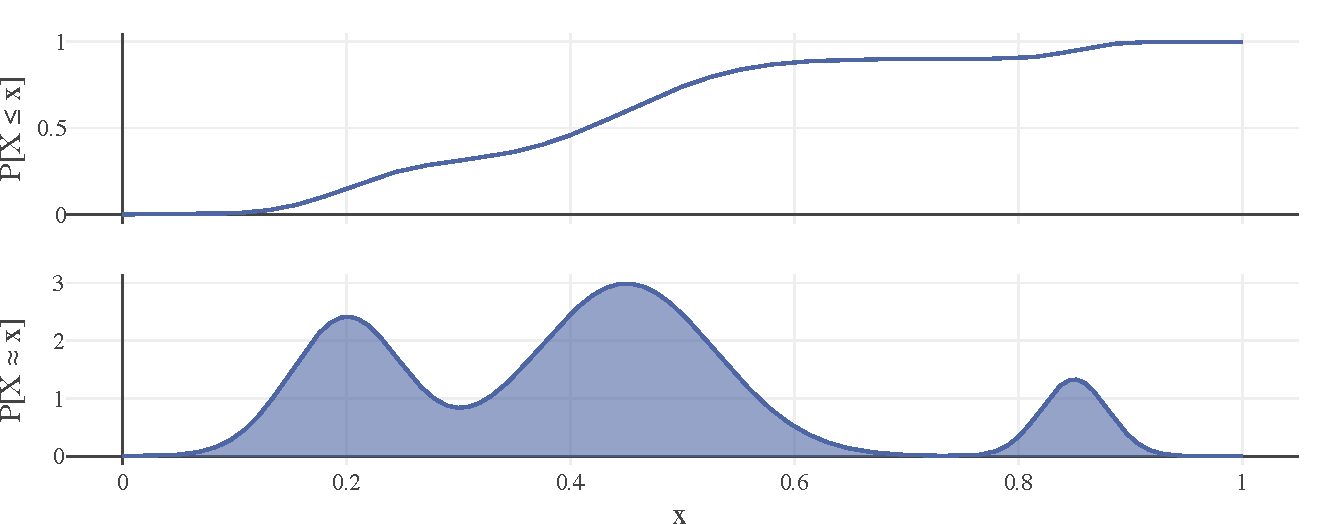
\includegraphics[width=.8\textwidth]{experiment_2_distribution}
%%   \caption{The cumulative distribution function (top) and
%%   probability density function (bottom) for the Gaussian mixture
%%   distribution in Experiment 2. The distributions have weights
%%   $(.3, .6, .1)$, means $(.2, .45, .85)$ and standard deviations
%%   $(.05, .08, .03)$. Random samples are generated from this mixture
%%   distribution by evaluating the inverse of the CDF at random
%%   numbers uniformly distributed in the range $[0,1]$.}
%% \end{figure}

%% \begin{figure}
%%   \centering
%%   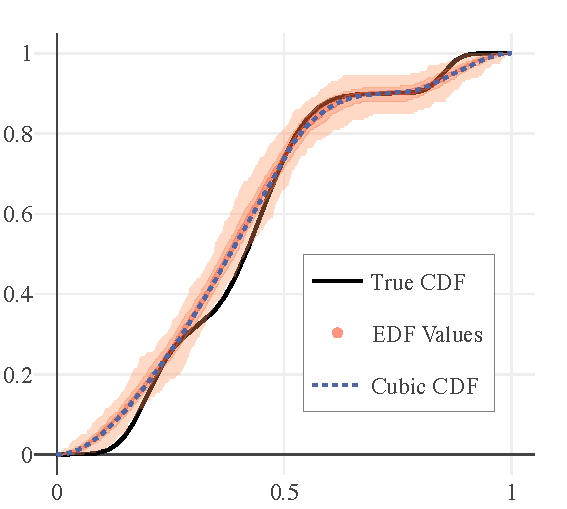
\includegraphics[width=.4\textwidth]{experiment_2_cubic_dist}
%%   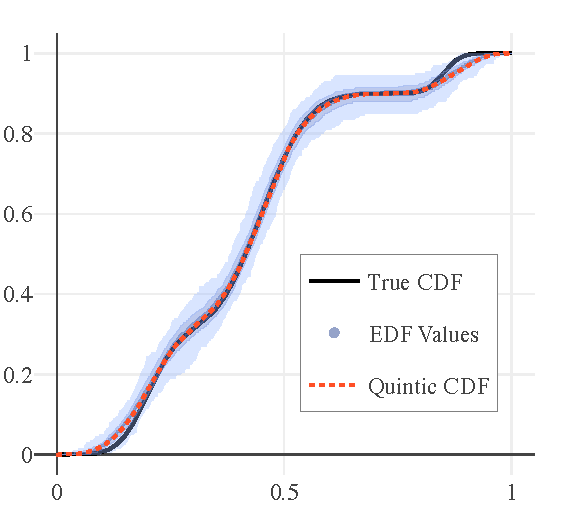
\includegraphics[width=.4\textwidth]{experiment_2_quintic_dist}
%%   \caption{Both cubic and quintic splines are used to approximate
%%   the CDF of a Gaussian mixture distribution with three
%%   components. Four CDF points are used to build the approximation,
%%   $200$ random samples are generated with the approximate CDFs over
%%   $100$ trials. The resulting cloud of empirical distribution
%%   function (EDF) values is seen above. The maximum approximation
%%   error in the CDFs are similar, $.08$ for the cubic and $.05$ for
%%   the quintic. However, the maximum EDF differences observed are
%%   doubled by the variance of random samples, $.15$ for the cubic
%%   and $.1$ for the quintic.}
%% \end{figure}

%% - generate large sets of random monotone data, show Table of number
%%   of metrics growing with increasing number of points

%% - show visual of the \textit{error} 

\heading{3.3 \enspace Random Monotone Data}

This experiment studies the number of times the algorithms {\tt
  is\_monotone} and {\tt make\_monotone} are executed for increasingly
large sequences of random monotone data. The minimum, median, and
maximum number of times that Algorithms \ref{alg:check-monotone} and
\ref{alg:make-monotone} are executed is recorded, as well as the
number of steps taken in all calls to {\tt binary\_search}. The number
of calls and steps grows linearly with $n$ as expected, requiring
roughly one call to {\tt make\_monotone} and $20$ binary search steps
to create a monotone piece. Some (less common) problems require an
average of three calls to {\tt make\_monotone} per interval.

%% \begin{table}
%%   \centering
%%   \caption{The minimum, median, and maximum number of checks,
%%   fixes, and binary search steps required in the execution of {\tt
%%   make\_spline} for increasing size sequences, $n$, over $100$
%%   randomly generated sets of monotone data. Notice the maximum for
%%   each counter is often significantly greater than the minimum and
%%   median, because the distribution of each counter is skewed
%%   right.}
%%   \begin{tabular}{c|c c c|c c c|c c c}
%%     \hline
%%     \multirow{2}{*}{$n$}
%%       & \multicolumn{3}{c|}{Checks} & \multicolumn{3}{c}{Fixes} & \multicolumn{3}{|c}{Search Steps} \\
%%       & min & median & max & min & median & max & min & median & max \\
%%     \hline
%%     5 & 4 & 6 & 274 & 0 & 1 & 154 & 3 & 31 & 2006\\
%%     25 & 28 & 47 & 378 & 2 & 14 & 225 & 80 & 348 & 3742\\
%%     50 & 61 & 124 & 484 & 6 & 40 & 238 & 217 & 851 & 4445\\
%%     75 & 102 & 216 & 842 & 14 & 74 & 411 & 463 & 1491 & 6333\\
%%     100 & 142 & 306 & 776 & 21 & 107 & 380 & 629 & 2140 & 7414\\
%%     \hline
%%   \end{tabular}
%% \end{table}
